\documentclass[12pt,letterpaper]{article}

% ─── Paquetes ────────────────────────────────────────────────────────────────
\usepackage[utf8]{inputenc}
\usepackage[T1]{fontenc}
\usepackage[spanish]{babel}
\usepackage[margin=2.5cm]{geometry}
\usepackage{graphicx}
\usepackage{xcolor}
\usepackage{booktabs}
\usepackage{array}
\usepackage{tabularx}
\usepackage{longtable}
\usepackage{enumitem}
\usepackage{amssymb}
\usepackage{pifont}
\usepackage{fancyhdr}
\usepackage{titlesec}
\usepackage{hyperref}
\usepackage{parskip}
\usepackage{listings}
\usepackage{float}

% ─── Colores ─────────────────────────────────────────────────────────────────
\definecolor{tecblue}{RGB}{0,70,127}
\definecolor{tecred}{RGB}{200,0,0}
\definecolor{codebg}{RGB}{245,247,250}
\definecolor{accentgreen}{RGB}{30,180,100}

% ─── Encabezado / pie ────────────────────────────────────────────────────────
\pagestyle{fancy}
\fancyhf{}
\fancyhead[L]{\small CE-5507 Modelación Hardware/Software OO}
\fancyhead[R]{\small LinProd — Documentación Técnica}
\fancyfoot[C]{\thepage}
\renewcommand{\headrulewidth}{0.4pt}

% ─── Secciones ───────────────────────────────────────────────────────────────
\titleformat{\section}{\bfseries\large\color{tecblue}}{}{0em}{}[\titlerule]
\titleformat{\subsection}{\bfseries\normalsize\color{tecblue!80}}{}{0em}{}
\titleformat{\subsubsection}{\bfseries\normalsize}{}{0em}{}

% ─── Listings ────────────────────────────────────────────────────────────────
\lstset{
  language=Python,
  backgroundcolor=\color{codebg},
  basicstyle=\ttfamily\small,
  keywordstyle=\bfseries\color{tecblue},
  commentstyle=\itshape\color{gray},
  numbers=none,
  frame=single,
  breaklines=true,
  tabsize=4,
  aboveskip=6pt, belowskip=6pt,
}

\newcommand{\cmark}{\textcolor{accentgreen}{\ding{51}}}
\newcommand{\xmark}{\textcolor{red}{\ding{55}}}
\newcolumntype{C}[1]{>{\centering\arraybackslash}p{#1}}

% ═════════════════════════════════════════════════════════════════════════════
\begin{document}

% ─── Portada ─────────────────────────────────────────────────────────────────
\begin{titlepage}
\centering
\vspace*{2cm}
{\large\bfseries Instituto Tecnológico de Costa Rica}\\[0.3em]
{\large Escuela de Ingeniería en Computadores}\\[0.3em]
{\normalsize CE-5507 — Modelación Hardware Software Orientado a Objetos}\\[0.3em]
{\normalsize I Semestre 2026}\\[2cm]
{\Huge\bfseries\color{tecred} LinProd}\\[0.5em]
{\LARGE\bfseries\color{tecblue} Documentación Técnica del Proyecto 2}\\[2cm]
\begin{tabular}{l}
  \toprule
  \textbf{Integrantes} \\
  \midrule
  Carlos Eduardo Zaldaña Lima \\
  Maria Laura Iglesias Gutierrez \\
  Yendry Melissa Calderón Gómez \\
  José Andrés Vargas Torres \\
  \bottomrule
\end{tabular}\\[2cm]
{\normalsize Fecha de entrega: 16 de mayo de 2026}
\end{titlepage}

\tableofcontents
\newpage

% ─────────────────────────────────────────────────────────────────────────────
\section{Diagrama de Clases}
% ─────────────────────────────────────────────────────────────────────────────

La Figura~\ref{fig:diagrama} muestra el diagrama UML de clases del sistema LinProd.
El sistema está organizado en cuatro módulos con dependencias estrictamente unidireccionales:
\texttt{model.py} $\leftarrow$ \texttt{simulator.py} $\leftarrow$ \{\texttt{app.py}, \texttt{reports.py}\}.

\begin{figure}[H]
  \centering
  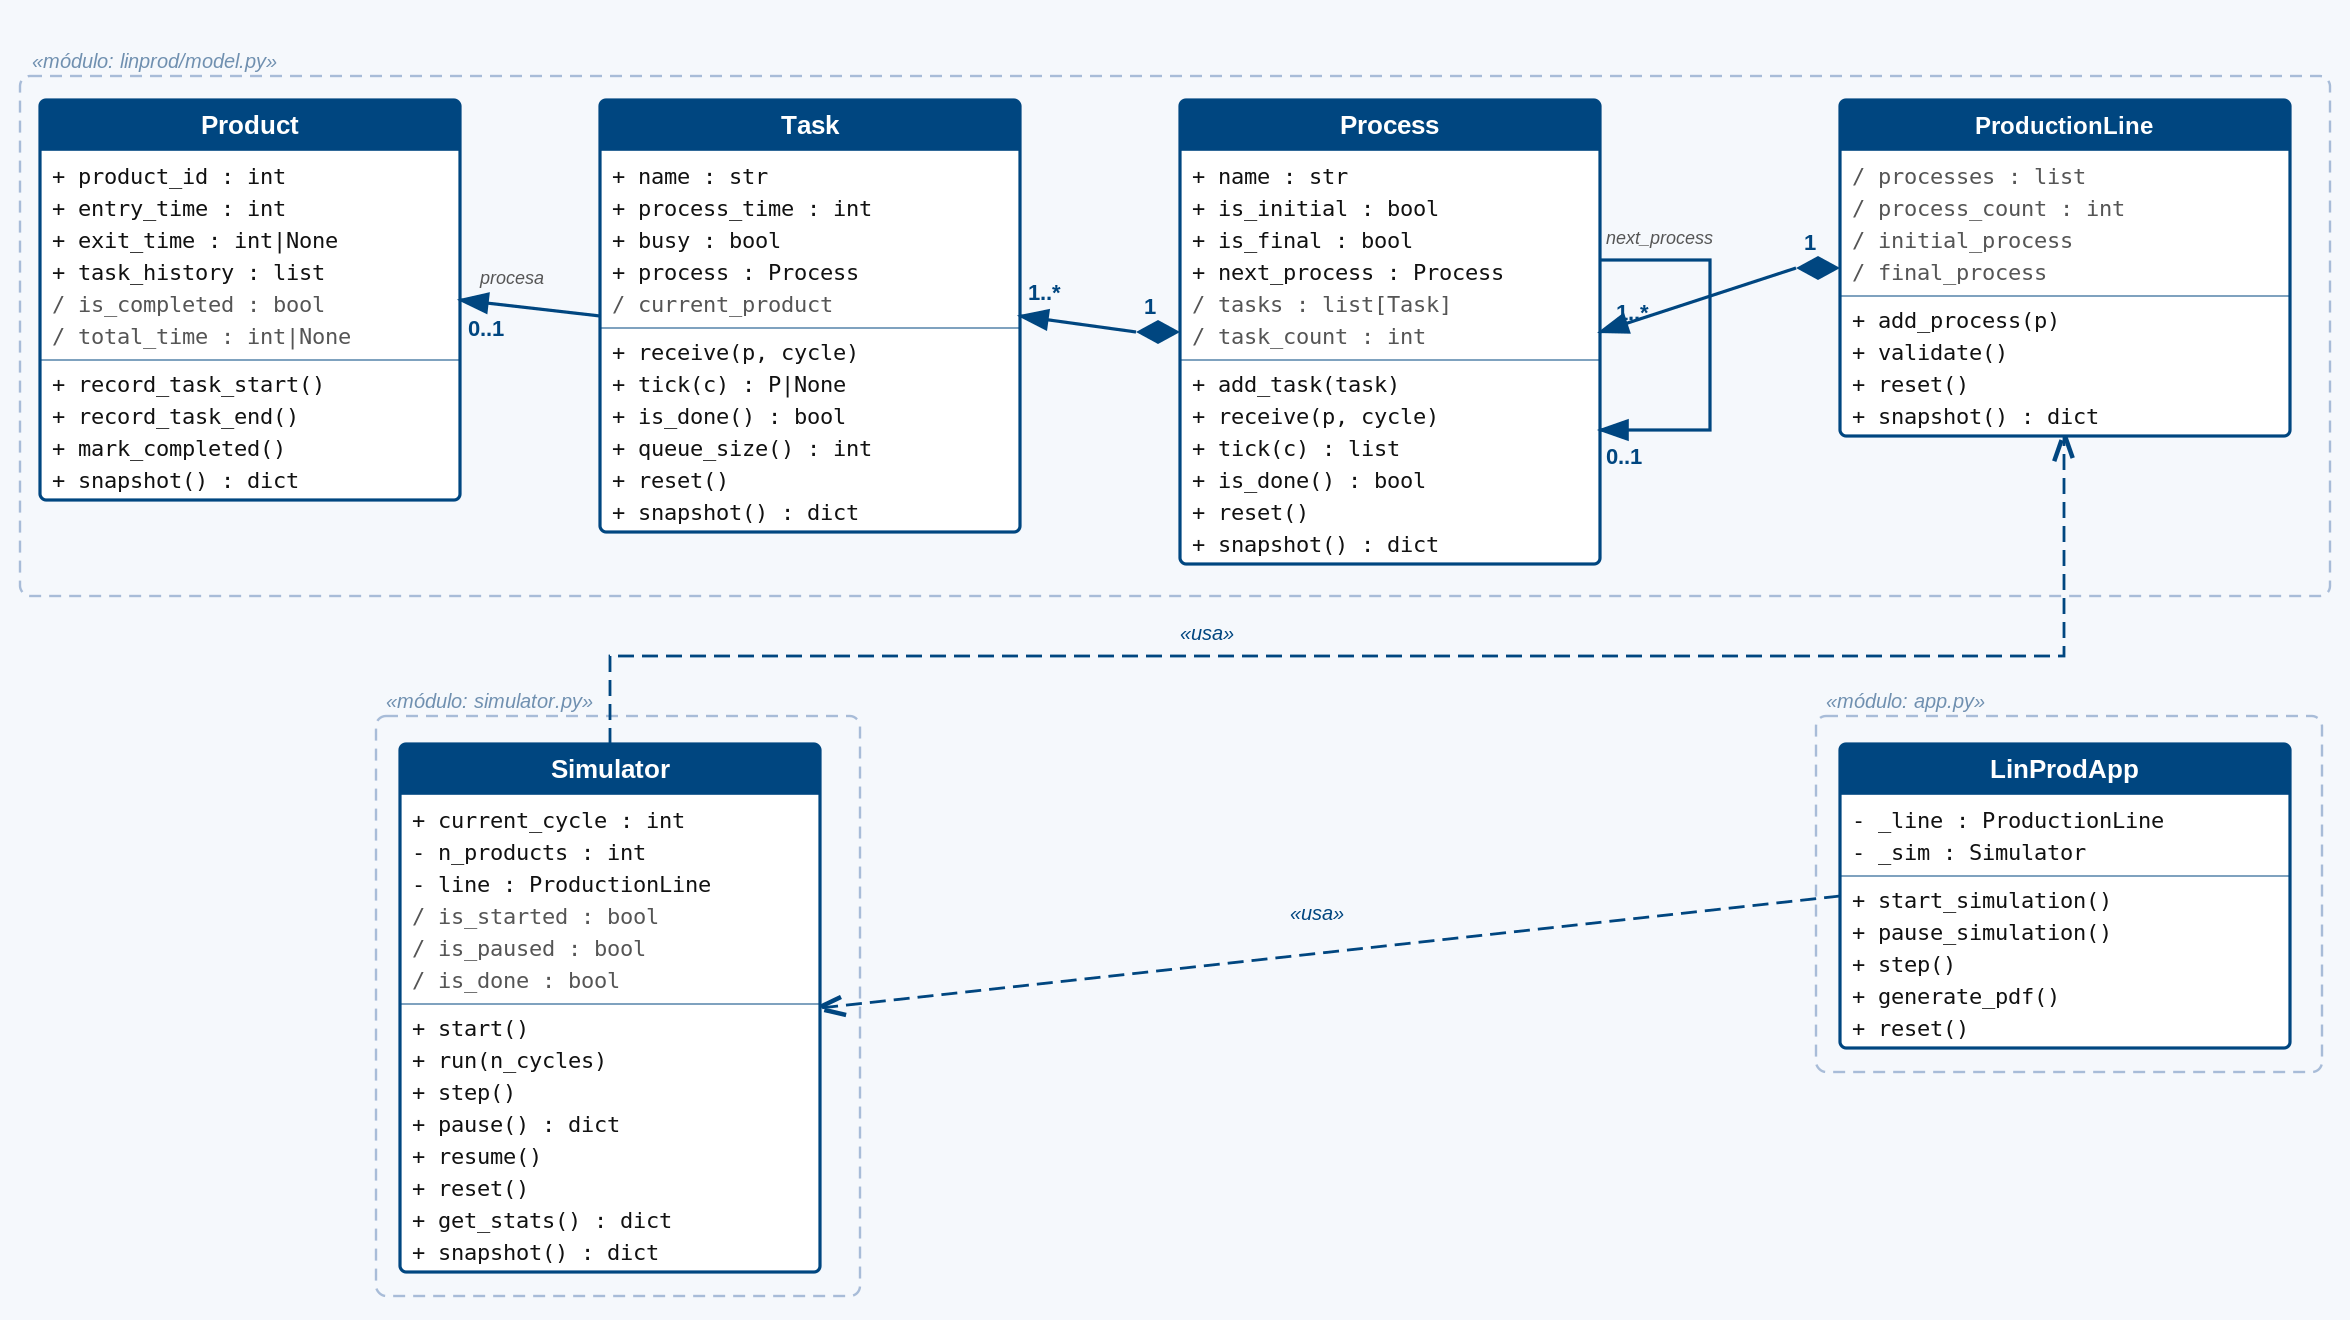
\includegraphics[width=\textwidth]{diagrama.png}
  \caption{Diagrama de clases del sistema LinProd.
           Notación: diamante relleno = composición, flecha sólida = asociación,
           flecha punteada = dependencia (\textit{«usa»}).
           Los atributos con \texttt{/} son propiedades derivadas de solo lectura.}
  \label{fig:diagrama}
\end{figure}

\subsection{Descripción de las clases principales}

\begin{description}[leftmargin=2em, labelindent=0em]
  \item[\texttt{Product}] Representa un producto que recorre la línea. Almacena
    su historial de paso por cada tarea (\texttt{task\_history}) y calcula el
    tiempo total de forma derivada.

  \item[\texttt{Task}] Modela una máquina con tiempo de procesamiento fijo. Atiende
    un producto a la vez; los demás esperan en una cola FIFO (\texttt{deque}).
    Lleva estadísticas de espera promedio usadas por el reporteador.

  \item[\texttt{Process}] Agrupa una lista ordenada de \texttt{Task}. Los productos
    atraviesan las tareas secuencialmente antes de salir al siguiente proceso.
    Mantiene referencia al proceso siguiente (\texttt{next\_process}).

  \item[\texttt{ProductionLine}] Cadena de \texttt{Process} validada: exactamente un
    proceso marcado como \texttt{is\_initial} y uno como \texttt{is\_final},
    cada uno con al menos una tarea.

  \item[\texttt{Simulator}] Motor de eventos discretos. Inyecta productos en el
    proceso inicial, avanza ciclo a ciclo y gestiona las transferencias entre
    procesos con semántica de \emph{pipeline real}: un producto que termina el
    proceso $N$ en el ciclo $K$ no entra al proceso $N+1$ hasta el ciclo $K+1$.

  \item[\texttt{LinProdApp}] Interfaz gráfica Tkinter (subclase de \texttt{tk.Tk}).
    Construye la \texttt{ProductionLine} a partir de la entrada del usuario y
    controla el \texttt{Simulator}. Incluye el botón de generación de PDF.
\end{description}

% ─────────────────────────────────────────────────────────────────────────────
\section{Alternativas de Solución Consideradas}
% ─────────────────────────────────────────────────────────────────────────────

\subsection{Framework de interfaz gráfica}

\begin{center}
\renewcommand{\arraystretch}{1.25}
\begin{tabularx}{\textwidth}{|l|X|X|C{1.8cm}|}
\hline
\textbf{Alternativa} & \textbf{Ventajas} & \textbf{Desventajas} & \textbf{Selección} \\
\hline
Tkinter &
  Incluido en la stdlib de Python, sin instalación adicional. Documentación amplia. Suficiente para el alcance del proyecto. &
  Apariencia anticuada por defecto; requiere estilos manuales para un diseño moderno. &
  \cmark\ Elegida \\
\hline
PyQt6 / PySide6 &
  Widgets más modernos, mayor control visual, Qt Designer. &
  Requiere \texttt{pip install pyqt6}. Licencia LGPL. Curva de aprendizaje mayor. &
  Descartada \\
\hline
wxPython &
  Apariencia nativa del sistema operativo. &
  Documentación más escasa, instalación más compleja en Linux. &
  Descartada \\
\hline
\end{tabularx}
\end{center}

Justificación: Tkinter fue elegida por ser parte de la distribución estándar de Python,
eliminando la necesidad de dependencias externas para la GUI. El diseño visual se modernizó
mediante widgets personalizados (\texttt{ModernButton}, \texttt{ModernEntry}, \texttt{Card})
con un tema oscuro implementado manualmente.

\subsection{Arquitectura del motor de simulación}

\begin{center}
\renewcommand{\arraystretch}{1.25}
\begin{tabularx}{\textwidth}{|l|X|X|C{1.8cm}|}
\hline
\textbf{Alternativa} & \textbf{Ventajas} & \textbf{Desventajas} & \textbf{Selección} \\
\hline
OOP ciclo-a-ciclo &
  Mapeo natural al dominio (productos, tareas, procesos como objetos). Fácil de depurar ciclo a ciclo. Determinismo garantizado. &
  Menos eficiente que una cola de eventos para sistemas con muchos eventos dispersos. &
  \cmark\ Elegida \\
\hline
Cola de eventos (\texttt{heapq}) &
  Mayor eficiencia en sistemas grandes (salta ciclos vacíos). Estándar en simuladores industriales. &
  Complejidad adicional; difícil de implementar correctamente en el tiempo disponible. &
  Descartada \\
\hline
Loop imperativo &
  Implementación simple. &
  Difícil de mantener; viola el principio OOP del enunciado. &
  Descartada \\
\hline
\end{tabularx}
\end{center}

Justificación: El enfoque OOP ciclo-a-ciclo se seleccionó porque mapea directamente
al enunciado del proyecto (el tiempo se mide en ciclos $t$) y facilita la generación del snapshot
de estado en cualquier ciclo, requerido para la funcionalidad de pausa.

\subsection{Orden de tick dentro de un proceso}

Este es el diseño más sutil del proyecto. Dentro de \texttt{Simulator.\_advance\_one\_cycle()},
las tareas de cada proceso se iteran en orden inverso (última $\to$ primera).

\begin{center}
\renewcommand{\arraystretch}{1.25}
\begin{tabularx}{\textwidth}{|l|X|X|C{1.8cm}|}
\hline
\textbf{Orden} & \textbf{Comportamiento} & \textbf{Problema} & \textbf{Selección} \\
\hline
Inverso (última → primera) &
  Una tarea que entrega su producto a la siguiente ya no es ticked de nuevo ese ciclo (la siguiente ya se procesó). Semántica de pipeline correcta. &
  Contra-intuitivo; requiere comentario explicativo. &
  \cmark\ Elegida \\
\hline
Directo (primera → última) &
  Orden natural. &
  Cuando T1 termina y entrega a T2, T2 es ticked inmediatamente en la misma iteración. El producto consume un ciclo de T2 en el mismo ciclo en que llegó: \emph{doble-tick}. &
  Descartada \\
\hline
\end{tabularx}
\end{center}

Justificación: Con tick inverso, T2 ya ha sido procesada cuando T1 le entrega el producto,
por lo que el producto recién recibido espera hasta el ciclo siguiente. Esto reproduce la semántica
real de una línea de montaje y produce los valores de referencia correctos:
Producto 1 = ciclo 12, Producto 2 = ciclo 16, Producto 3 = ciclo 20 (verificado con 65 pruebas).

\subsection{Librería de generación de PDF}

\begin{center}
\renewcommand{\arraystretch}{1.25}
\begin{tabularx}{\textwidth}{|l|X|X|C{1.8cm}|}
\hline
\textbf{Alternativa} & \textbf{Ventajas} & \textbf{Desventajas} & \textbf{Selección} \\
\hline
reportlab &
  Control total sobre el diseño. Mencionada explícitamente en la guía del proyecto. API estable y madura. &
  La fuente por defecto (Helvetica) no soporta UTF-8; requiere registrar DejaVu. &
  \cmark\ Elegida \\
\hline
fpdf2 &
  API más simple. Soporte UTF-8 nativo. &
  Menos control sobre tablas complejas. &
  Descartada \\
\hline
pdfkit / weasyprint &
  Genera PDF desde HTML/CSS. &
  Requiere binario externo (\texttt{wkhtmltopdf}). Mayor complejidad de instalación. &
  Descartada \\
\hline
\end{tabularx}
\end{center}

% ─────────────────────────────────────────────────────────────────────────────
\section{Problemas Conocidos}
% ─────────────────────────────────────────────────────────────────────────────

Al momento de la entrega no se conocen problemas abiertos en el sistema.
Las 65 pruebas automatizadas pasan, la GUI funciona con líneas de hasta $N$ procesos ilimitados,
y el reporte PDF se genera correctamente para todas las configuraciones probadas.

Si el sistema no tiene la fuente DejaVu instalada en
\texttt{/usr/share/fonts/truetype/dejavu/}, el reporte PDF usa Helvetica como
respaldo, lo que puede causar que los caracteres con tilde ($á$, $é$, $ñ$, etc.)
no se muestren en el PDF. El programa \emph{no falla}; simplemente degrada la
tipografía. Solución: instalar las fuentes con
\texttt{sudo apt-get install fonts-dejavu}.

% ─────────────────────────────────────────────────────────────────────────────
\section{Problemas Encontrados}
% ─────────────────────────────────────────────────────────────────────────────

\subsection{Problema 1: Doble-tick de productos dentro de un proceso}

\subsubsection*{Descripción}

Durante el desarrollo del motor de simulación (\texttt{simulator.py}), se detectó que
los productos terminaban antes de lo esperado según los valores de referencia del enunciado.
Con la línea de referencia (Ensamblado $\to$ Pintura $\to$ Control), el Producto 1 salía en
el ciclo 11 en lugar del ciclo 12 correcto.

\subsubsection*{Diagnóstico}

Al simular con iteración directa (tarea 1 $\to$ tarea 2), cuando la Tarea 1 terminaba en el
ciclo $K$ y entregaba el producto a la Tarea 2, el bucle inmediatamente ticked a la Tarea 2
en ese mismo ciclo $K$. El producto recibía un ciclo gratuito de procesamiento, adelantando
todos los tiempos de salida en un ciclo.

\begin{lstlisting}
# Código problemático (orden directo - primer intento):
for i, task in enumerate(tasks):
    finished = task.tick(current_cycle)
    if finished and i < n_tasks - 1:
        tasks[i+1].receive(finished, current_cycle)
        # tasks[i+1] también será ticked en esta misma iteración
\end{lstlisting}

\subsubsection*{Intentos de solución sin éxito}

\begin{enumerate}[leftmargin=2em]
  \item Diferir la entrega un ciclo con lista temporal: se intentó guardar los
    productos a entregar en una lista \texttt{pending\_intra} y aplicarlos al inicio del
    siguiente ciclo. Esto corregía el problema intra-proceso pero rompía la semántica
    inter-proceso (ahora había dos ciclos de retardo en lugar de cero intra y uno inter).
  \item Marcar tareas como «recién cargadas»: se añadió una bandera \texttt{just\_received}
    en \texttt{Task.receive()} para que \texttt{tick()} no procesara en el mismo ciclo.
    Funcionó pero introdujo estado compartido de difícil mantenimiento y falló con colas.
\end{enumerate}

\subsubsection*{Solución encontrada}

Iterar las tareas en orden inverso dentro de cada proceso:

\begin{lstlisting}
# Solución: orden inverso (última → primera tarea)
for i in range(n_tasks - 1, -1, -1):
    task = tasks[i]
    finished = task.tick(self.current_cycle)
    if finished is not None:
        if i == n_tasks - 1:
            # salió del proceso completo
            new_pending.append((finished, proc.next_process))
        else:
            # entrega a la siguiente tarea
            tasks[i + 1].receive(finished, self.current_cycle)
            # tasks[i+1] ya fue ticked antes en esta iteración
\end{lstlisting}

Al tickear de último a primero, cuando la Tarea 1 (índice 0) entrega a la Tarea 2 (índice 1),
la Tarea 2 ya terminó su tick en esta iteración y no recibirá otro hasta el siguiente ciclo.

\subsubsection*{Verificación}

La prueba de referencia confirma la solución:
\begin{lstlisting}
assert by_id[1]["exit_time"] == 12  # Producto 1
assert by_id[2]["exit_time"] == 16  # Producto 2
assert by_id[3]["exit_time"] == 20  # Producto 3
\end{lstlisting}

\subsubsection*{Recomendación}

Al diseñar simuladores de pipeline ciclo-a-ciclo, el orden de tick de los elementos es
un invariante no trivial. Se recomienda documentarlo con un comentario en el código y
cubrirlo explícitamente con una prueba (ver \texttt{test\_reverse\_tick\_order\_within\_process}).

\vspace{0.8em}
\subsection{Problema 2: Error \texttt{ModuleNotFoundError} al ejecutar scripts directamente}

\subsubsection*{Descripción}

Al ejecutar \texttt{python3 linprod/simulator.py} desde la raíz del repositorio, Python
lanzaba \texttt{ModuleNotFoundError: No module named 'linprod'} porque los imports
relativos (\texttt{from linprod.model import ...}) no resuelven correctamente cuando el
script se ejecuta como archivo plano.

\subsubsection*{Solución encontrada}

Ejecutar los módulos como paquete usando la bandera \texttt{-m}:

\begin{lstlisting}[language=bash]
python3 -m linprod.simulator   # correcto
python3 linprod/simulator.py   # falla
\end{lstlisting}

Los comandos de prueba del proyecto (incluyendo \texttt{python3 -m linprod.app} para la
GUI y \texttt{python3 -m linprod.reports} para el reporte) usan consistentemente esta
convención.

\vspace{0.8em}
\subsection{Problema 3: Soporte de UTF-8 en reportlab}

\subsubsection*{Descripción}

Al generar el reporte PDF con la fuente por defecto \texttt{Helvetica}, los caracteres con
tilde y la letra ñ aparecían como signos de interrogación o caracteres corruptos en el PDF.

\subsubsection*{Diagnóstico}

La fuente Helvetica (fuente Type 1 integrada en reportlab) no incluye el mapa de caracteres
extendido de Latin-1/UTF-8. Cualquier carácter fuera del ASCII básico falla silenciosamente.

\subsubsection*{Solución encontrada}

Registrar la fuente TrueType \texttt{DejaVuSans} antes de construir el documento:

\begin{lstlisting}
from reportlab.pdfbase import pdfmetrics
from reportlab.pdfbase.ttfonts import TTFont

_DEJAVU_PATHS = [
    "/usr/share/fonts/truetype/dejavu/DejaVuSans.ttf",
    "/usr/share/fonts/dejavu/DejaVuSans.ttf",
]

def _register_fonts():
    for path in _DEJAVU_PATHS:
        if os.path.exists(path):
            pdfmetrics.registerFont(TTFont("DejaVu", path))
            return "DejaVu"
    return "Helvetica"   # fallback
\end{lstlisting}

\subsubsection*{Recomendación}

Siempre registrar una fuente TTF con soporte Unicode en proyectos reportlab que usen
español. La ruta más portátil en sistemas Debian/Ubuntu es
\texttt{/usr/share/fonts/truetype/dejavu/DejaVuSans.ttf}.

\vspace{0.8em}
\subsection{Problema 4: \texttt{sim.run()} requería argumento obligatorio}

\subsubsection*{Descripción}

La guía del Módulo 2 mostraba el uso de \texttt{sim.run()} sin argumentos para
«correr hasta terminar», pero la firma original era \texttt{def run(self, n\_cycles: int)},
lo que hacía \texttt{n\_cycles} obligatorio y lanzaba \texttt{TypeError} al omitirlo.

\subsubsection*{Solución}

Se añadió un valor por defecto de 100\,000 ciclos:

\begin{lstlisting}
def run(self, n_cycles: int = 100_000) -> None:
    ...
    for _ in range(n_cycles):
        if self._paused or self.is_done:
            break
        self._advance_one_cycle()
\end{lstlisting}

El loop rompe antes de llegar al límite si \texttt{is\_done} se activa, por lo que en la
práctica \texttt{run()} sin argumento equivale a «correr hasta que todos los productos
completen la línea».

% ─────────────────────────────────────────────────────────────────────────────
\section{Conclusiones y Recomendaciones}
% ─────────────────────────────────────────────────────────────────────────────

\subsection{Conclusiones}

\begin{enumerate}[leftmargin=2em, itemsep=6pt]
  \item El paradigma OOP es adecuado para simulación de líneas de producción.
    La correspondencia directa entre los objetos del dominio (productos, tareas, procesos)
    y las clases Python redujo la brecha entre el modelo conceptual y la implementación,
    facilitando el diseño, la depuración y las pruebas.

  \item Los invariantes sutiles del motor de simulación deben documentarse y
    probarse explícitamente. El orden inverso de tick es un detalle no obvio que, si se
    rompe, produce resultados incorrectos sin errores visibles. La prueba
    \texttt{test\_reverse\_tick\_order\_within\_process} es la salvaguarda crítica.

  \item La cobertura de pruebas (65 pruebas) brinda confianza en el determinismo.
    La prueba de referencia contra los valores del enunciado (P1=12, P2=16, P3=20) actúa
    como \emph{golden test}: cualquier regresión en la lógica central lo romperá primero.

  \item La separación estricta de módulos (model $\leftarrow$ simulator $\leftarrow$
    app/reports) facilita el trabajo en paralelo. Cada módulo pudo desarrollarse y probarse
    de forma independiente, reduciendo conflictos de integración.

  \item Reportlab es potente pero requiere atención al soporte de caracteres.
    La gestión de fuentes TTF es un paso adicional necesario para producir documentos
    profesionales en español con tildes y ñ.
\end{enumerate}

\subsection{Recomendaciones}

\begin{enumerate}[leftmargin=2em, itemsep=6pt]
  \item Mantener el invariante de tick inverso documentado. Si en el futuro se necesita
    soporte para procesos con semántica diferente (e.g., tareas en paralelo dentro de un
    proceso), rediseñar esa parte sin comprometer el tick inverso de las tareas secuenciales.

  \item Extender la suite de pruebas con líneas de 5+ procesos para cubrir el escenario
    exacto que el profesor presentará en la defensa.

  \item Considerar exportar el snapshot de pausa en formato JSON para facilitar la
    depuración y la revisión post-ejecución.

  \item Para producción real, reemplazar el límite de 100\,000 ciclos en \texttt{run()}
    por detección explícita de \emph{deadlock} (todos los procesos sin movimiento por
    N ciclos consecutivos).
\end{enumerate}

% ─────────────────────────────────────────────────────────────────────────────
\section{Bibliografía}
% ─────────────────────────────────────────────────────────────────────────────

\begin{enumerate}[leftmargin=2em, label={[\arabic*]}]

  \item Instituto Tecnológico de Costa Rica. \textit{Enunciado del Proyecto 2 — LinProd}.
    CE-5507 Modelación Hardware Software Orientado a Objetos, I Semestre 2026.

  \item Python Software Foundation. \textit{The Python Standard Library — tkinter:
    Python interface to Tcl/Tk}. Disponible en: \url{https://docs.python.org/3/library/tkinter.html}
    [Acceso: mayo 2026].

  \item Python Software Foundation. \textit{collections.deque — Double-ended queue}.
    Disponible en: \url{https://docs.python.org/3/library/collections.html#collections.deque}
    [Acceso: mayo 2026].

  \item ReportLab Inc. \textit{ReportLab PDF Library User Guide}. Disponible en:
    \url{https://www.reportlab.com/docs/reportlab-userguide.pdf} [Acceso: mayo 2026].

  \item Wikipedia. \textit{Producción en cadena}. Disponible en:
    \url{https://es.wikipedia.org/wiki/Produccion_en_cadena} [Acceso: mayo 2026].
    (Fuente citada en el marco teórico del enunciado.)

  \item Wikipedia. \textit{Discrete-event simulation}. Disponible en:
    \url{https://en.wikipedia.org/wiki/Discrete-event_simulation} [Acceso: mayo 2026].

  \item Law, A. M. \textit{Simulation Modeling and Analysis}, 5th ed. McGraw-Hill, 2015.
    Cap. 1 y 2: fundamentos de simulación de eventos discretos.

  \item pytest Development Team. \textit{pytest: helps you write better programs}.
    Disponible en: \url{https://docs.pytest.org} [Acceso: mayo 2026].

\end{enumerate}

\end{document}
